\documentclass[11pt]{beamer}
\input{src/packages/fontenc}                % per il font
\input{src/packages/inputenc}               % per l'input
\input{src/packages/babel}                  % lingua principale inglese, secondaria italiano
\usepackage{amsmath}
\input{src/packages/amsfonts}               % cose utili per fare matematica e fisica
\input{src/packages/amssymb}                % intlimits mette gli estremi di integrazione sopra e sotto il segno di integrale       
\input{src/packages/amsthm}                 % cose utili per fare matematica e fisica
\input{src/packages/bbm}                    % cose utili per fare matematica e fisica
\input{src/packages/physics}                % cose utili per fare matematica e fisica
\input{src/packages/tensor}                 % =======================================
\input{src/packages/siunitx}
\input{src/packages/graphicx}               % per le foto
\input{src/packages/tikz}                   % per fare i disegnini belli
\input{src/packages/pgf}
\input{src/packages/pgfplots}
\input{src/packages/enumitem}               % 
\input{src/packages/lettrine}               % per le lettere belle a inizio capitolo
% \usepackage{hyperref}

% >> settings:

\hypersetup{                    
    colorlinks=true,       
    linkcolor=black,       
    filecolor=black,       
    urlcolor=blue,         
    pdfpagemode=FullScreen,
    citecolor=black,       
}
        
\input{src/packages/pifont}

\input{src/packages/xurl}
\input{src/packages/csquotes}
\usepackage[backend = bibtex, style = numeric-comp, maxbibnames = 5]{biblatex}

% >> settings:

\addbibresource{assets/references.bib}

\usepackage{src/packages/my-science-utils}
\usepackage{src/packages/my-thesis-utils}

\usefonttheme{serif}

\definecolor{CTgreen}{HTML}{28794e} % Catania green (primary)


\mode<presentation>
{
  \usetheme{Warsaw} 
  % \usetheme{Madrid}
  % \usetheme{Montpellier}
  % \usetheme{Marburg} 
  \usecolortheme[named=CTgreen]{structure}
  \setbeamercolor{alerted text}{fg=CTgreen}
  \setbeamercovered{transparent}
  \setbeamertemplate{section in toc}[ball unnumbered]
}

\expandafter\def\expandafter\insertshorttitle\expandafter{%
  \insertshorttitle\hfill%
  \insertframenumber\,/\,\inserttotalframenumber}

\newcommand{\backupbegin}{
   \newcounter{framenumberappendix}
   \setcounter{framenumberappendix}{\value{framenumber}}
}
\newcommand{\backupend}{
   \addtocounter{framenumberappendix}{-\value{framenumber}}
   \addtocounter{framenumber}{\value{framenumberappendix}} 
}

\newcommand{\refer}[1]{%
   \begin{flushright}
      {\alert{\tiny #1}}
   \end{flushright}}
  
\newcommand{\lrefer}[1]{%
   \begin{flushleft}
      {\alert{\tiny #1}}
   \end{flushleft}}
  
\newcommand{\param}[1]{%
   \begin{flushright}
      {\small #1}
   \end{flushright}
   \vspace{-1.5\baselineskip}
}

\newcommand{\etal}{{\em et al.}}




\title[Non-Hermitian Quantum Mechanics]{Non-Hermitian Quantum Mechanics}

\author[A. Pappalardo]{\large{Aurelio Pappalardo}}

\institute[DFA.UniCT]{
\begin{minipage}[c]{1.5truecm}
    \includegraphics[width=\textwidth]{logo_ellipse}
\end{minipage}
\begin{minipage}[c]{4truecm}
    \begin{flushleft}
        \begin{sl}
        Dipartimento di Fisica e Astronomia\\ 
        ``Ettore Majorana''
        \end{sl}
    \end{flushleft}
\end{minipage}
\begin{minipage}[c]{2.6truecm}
    \includegraphics[width=\textwidth]{logo_unict_orizzontale}
\end{minipage}}

\date{}

\begin{document}

    \begin{frame}[plain]
        \titlepage
    \end{frame}

    \begin{frame}[label=outline]
        \frametitle{Outline}
        \tableofcontents[pausesections]
    \end{frame}

    \section{Operatori Hermitiani}
\begin{frame}{Osservabili fisiche}
    Nella Meccanica Quantistica standard, gli stato fisico $\ket{\psi}$ è un vettore in uno spazio di Hilbert \mcH. Le quantità osservabili sono associate ad operatori Hermitiani su \mcH.

    \pause
    Il processo di misura di un'osservabile \hA :
    \begin{enumerate}[label=\mybullet]
        \pause
        \item Distrugge lo stato fisico $\ket{\psi}$;
        \pause
        \item Fa collassare il sistema nell'autostato $\ket{\phi_n}$ di \hA\ associato all'autovalore $\lambda_n$.
        \pause
        \item Restituisce come misura l'autovalore $\lambda_n$ di \hA;
    \end{enumerate}
    \pause
    La misura è un fenomeno aleatorio, la probabilità di osservare l'autovalore $\lambda_n$ è
    \begin{equation*}
        P\pqty{\lambda_n} = \abs{\braket{\phi_n}{\psi}}^2
    \end{equation*}
    \refer{A.N. \etal, PRB (2019)}
\end{frame}

\begin{frame}
    Come mai è importante che gli operatori siano Hermitiani?
    \begin{enumerate}[label=\mybullet]
        \pause
        \item Spettro reale:
            \begin{equation*}
                \hA\!\ket{\phi_n} = \lambda_n\!\ket{\phi_n}
                \quad\implies\quad
                \lambda_n \in \bbR
                \mycomma
            \end{equation*}
            essenziale affinché le misure abbiano senso fisico;
        \pause
        \item Autospazi ortogonali:
            \begin{equation*}
                \braket{\phi_m}{\phi_n} = \tensor{\delta}{_m_n}\mycomma
            \end{equation*}
            le possibili misure sono mutualmente esclusive;
        \pause
        \item Generano trasformazioni di simmetria:
            \begin{equation*}
                \hU = \myexp{i\hA}
                \quad\implies\quad
                \hU~\text{unitario}
                \myperiod
            \end{equation*}
    \end{enumerate}
\end{frame}


    \section{Operatori \hP, \hT\ e \hPT}
\begin{frame}{Il gruppo di Lorentz}
    Le trasformazioni di Lorentz sono quelle trasformazioni che lasciano invariato il 4-intervallo:
    \begin{equation*}
        \Delta s^2 = \tensor{x}{_\mu}\tensor{x}{^\mu} = c^2t^2 - x^2 - y^2 - z^2
        \myperiod
    \end{equation*}
    \pause
    I cambi di segno di una o più delle coordinate, come
    \begin{enumerate}[label=\mybullet]
        \item $ct \to -ct$
        \item $x \to -x$
        \item $\vb{r} \to -\vb{r}$, con $\vb{r} \equiv \pqty{x,y,z}$
    \end{enumerate}
    conservano il $4$-intervallo, quindi sono ancora trasformazioni di Lorentz.
\end{frame}

\begin{frame}{Trasformazioni \mcP\ e \mcT}
    Introduciamo due trasformazioni:
    \begin{enumerate}[label=\mybullet]
        \pause
        \item Inversione di parità, che inverte le coordinate spaziali:
            \begin{equation*}
                \func{\mcP}{\pqty{ct,\vb{r}}}{\pqty{ct,-\vb{r}}}
            \end{equation*}
        \pause
        \item Inversione temporale, che inverte il tempo
            \begin{equation*}
                \func{\mcT}{\pqty{ct,\vb{r}}}{\pqty{-ct,\vb{r}}}
            \end{equation*}
            \pause L'effetto dell'Inversione temporale in realtà è quello di invertire la direzione del moto.
    \end{enumerate}
\end{frame}

\begin{frame}{Connessione del gruppo di Lorentz}
    Le trasformazioni di Lorentz formano un gruppo e sono identificate dal parametro $\vb*{\beta} = \vb{v}/c$.

    \pause
    Il gruppo di Lorentz si divide in quattro componenti connesse:
    \begin{enumerate}[label=\mybullet]
        \pause
        \item Il sottogruppo contentente l'identità;
        \pause
        \item Il sottogruppo dell'identità composto con \mcP;
        \item Il sottogruppo dell'identità composto con \mcT;
        \item Il sottogruppo dell'identità composto con \mcP\mcT;
    \end{enumerate}
    \pause
    Queste quattro componenti sono sconnesse tra loro.
    
        
\end{frame}

\begin{frame}{Connessione del gruppo di Lorentz}
    Le componenti possono essere ridotte a due passando ai numeri complessi.
    \begin{figure}
        \begin{tikzpicture}
            \draw (1,1) -- (1,2);
        \end{tikzpicture}
        \qquad\pause
        \begin{tikzpicture}
            \draw (1,1) -- (2,1);
        \end{tikzpicture}
    \end{figure}
    \pause
    La componente dell'identità si connette alla componente \PT.
    \pause
    Le trasformazioni \PT\ potrebbero quindi avere un ruolo privilegiato.
\end{frame}

\begin{frame}{Passaggio agli operatori quantistici}
    Introduciamo gli operatori quantistici \hP\ e \hT, analoghi dei classici \mcP\ e \mcT :
    \begin{enumerate}[label=\mybullet]
        \pause
        \item L'inversione di parità inverte posizione e impulso, il sistema appare come allo specchio:
            \begin{equation*}
                \hP\hvr\hP^{-1} = -\hvr
                \mycomma
                \qquad
                \hP\hvp\hP^{-1} = -\hvp
                \mysemicolon
            \end{equation*}
        \pause
        \item L'inversione temporale inverte l'impulso ma non la posizione, il sistema appare come se si evolvesse a ritroso:
            \begin{equation*}
                \hT\hvr\hT^{-1} = \hvr
                \mycomma
                \qquad
                \hT\hvp\hT^{-1} = -\hvp
                \myperiod
            \end{equation*}
    \end{enumerate}
    \pause
    Si pone inoltre $\comm*{\hP}{\hT}\! = 0$.
\end{frame}

\begin{frame}{Linearità e antilinearità}
    Imponendo che le trasformazioni \hP\ e \hT\ lascino invariate le relazioni di commutazione canoniche
    \begin{equation*}
        \comm*{\tensor{\hx}{_j}}{\tensor{\hp}{_k}}\! = i\hbar\tensor{\delta}{_j_k}
        \mycomma
    \end{equation*}
    si trova che 
    \begin{enumerate}[label=\mybullet]
        \item \hP\ deve essere lineare, ovvero $\forall\ket{\psi},\ket{\phi}\in\mcH$, $\forall\lambda,\mu\in\bbC$
            $$
                \hP\pqty{\lambda\!\ket{\psi} + \mu\!\ket{\phi}}
                = \lambda\hP\!\ket{\psi} + \mu\hP\!\ket{\phi}
            $$
        \item \hT\ deve essere \emph{antilineare}, ovvero
            $$
                \hT\pqty{\lambda\!\ket{\psi} + \mu\!\ket{\phi}}
                = \lambda^*\hT\!\ket{\psi} + \mu^*\hT\!\ket{\phi}
            $$
    \end{enumerate}
\end{frame}

\begin{frame}{Proprietà di \hP}
    Si può inoltre dimostrare che \hP :
    \begin{enumerate}[label=\mybullet]
        \pause
        \item È Hermitiano $$\hP = \hP^\dag\mysemicolon$$
        \pause
        \item È unitario $$\hP^{-1} = \hP^\dag\mysemicolon$$
        \pause
        \item Il suo quadrato è l'identità $$\hP^2 = \hidM\myperiod$$
    \end{enumerate}
    \pause
    Di conseguenza, gli autovalori di \hP\ sono $\pm1$: $$\hP\!\ket{\pm} = \pm\!\ket{\pm}.$$
\end{frame}

\begin{frame}{Proprietà di \hT}
    Per \hT\ il discorso è più delicato. È un operatore \emph{antiunitario}
    Se trasformo due vettori
    $$\ket*{\psi'} = \hT\!\ket{\psi}\quad\text{e}\quad\ket*{\phi'} = \hT\!\ket{\phi}\mycomma$$
    \pause
    e ne faccio il prodotto scalare, ottengo il complesso coniugato:
    $$\braket*{\phi'}{\psi'} = \braket{\phi}{\psi}^*\myperiod$$
    \pause
    L'operatore \hT\ non conserva il prodotto scalare ma conserva il suo modulo
    $\abs*{\!\braket*{\phi'}{\psi'}}\! = \abs{\braket{\phi}{\psi}}$,
    essenziale per conservare la probabilità.

    \pause 
    Infine $\hT^2 = \hidM$ vale solo per i sistemi con spin intero.
\end{frame}

\begin{frame}{Operatore \hPT\ e sue proprietà}
    L'operatore \hPT\ è la composizione di \hP\ e \hT. Di conseguenza è antiunitario e per sistemi senza spin è tale che $\bqty*{\hPT}\!^2 = \hidM$.

    \pause
    Possiamo imporre che abbia autovalori uguali a $1$:
    $$
        \hPT\!\ket{\psi} = \lambda\!\ket{\psi}
        \quad\implies\quad
        \lambda = e^{i\theta}
        \mysemicolon
    $$
    Ridefiniamo $\ket*{\psi'} = e^{i\theta/2}\!\ket{\psi}$ e otteniamo
    $$
        \hPT e^{i\theta/2}\!\ket{\psi}
        =\pause e^{-i\theta/2}\hPT\!\ket{\psi}
        =\pause e^{-i\theta/2}e^{i\theta}\!\ket{\psi}
        =\pause e^{i\theta/2}\!\ket{\psi}
        \myperiod
    $$
    \pause
    da cui $$\hPT\!\ket*{\psi'} = \ket*{\psi'}$$
\end{frame}
    \section{Simmetria \PT\ e \CPT}
\begin{frame}{Operatori \PT-invarianti}
    Diciamo che un operatore è \hPT-invariante se
    $$\PTtransform{\hA} = \hA\mycomma$$
    o analogamente
    $$\comm*{\hPT}{\hA}\! = 0\myperiod$$
    \pause
    Se $\ket{\psi}$ è un autostato \emph{simultaneo} di \hA\ e \hPT, l'autovalore $\lambda$ di \hA\ associato a $\ket{\psi}$ è \emph{reale}, infatti
    \begin{align*} 
        \hPT\pqty*{\hA\!\ket{\psi}}\! = \hPT\pqty{\lambda\!\ket{\psi}}
        \quad&\iff\quad
        \pause
        \hA\hPT\!\ket{\psi} = \lambda^*\hPT\!\ket{\psi} \\
        \pause
        \hA\!\ket{\psi} = \lambda^*\!\ket{\psi}
        \quad&\iff\quad
        \lambda\!\ket{\psi} = \lambda^*\!\ket{\psi}
    \end{align*}
\end{frame}

\begin{frame}
    Domanda:
    \begin{center}
        {\it Esiste una classe più generale di operatori con autovalori reali?}
    \end{center}
    Risposta:
    \pause
    \begin{center}
        {\it Sì e no, perché non tutti gli operatori Hermitiani sono \emph{anche} \PT-invarianti, ma esistono operatori \emph{non Hermitiani} che hanno autovalori reali.}
    \end{center}
    \pause
    \begin{figure}
        \centering
        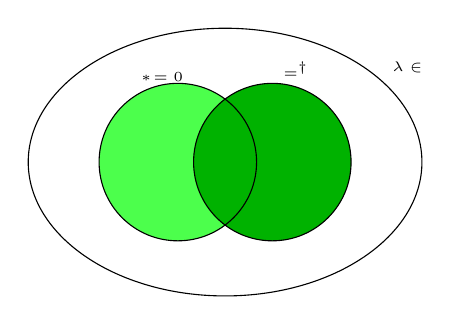
\begin{tikzpicture}
            \fill[color=green!70!white] (-0.6,0) circle (1);
            \fill[color=green!70!black] (0.6,0) circle (1);
            \draw (-0.6,0) circle (1);
            \draw (+0.6,0) circle (1);
            \draw (0,0) ellipse (2.5 and 1.7);
            \node[anchor=south] at (0.9,0.95) {\tiny{$\hH = \hH^\dag$}};
            \node[anchor=south, align=center] at (-0.8,0.9) {\tiny{$\comm*{\hPT}{\hH}\! = 0$}};
            \node[anchor=west, align=center] at (2,1.2) {\tiny{$\lambda\in\bbR$}};
        \end{tikzpicture}
    \end{figure}
\end{frame}

\begin{frame}{Simmetria \PT}
    Diciamo che un sistema fisico \emph{non rompe la Simmetria \PT} se
    \begin{enumerate}[label=\mybullet]
        \pause
        \item L'Hamiltoniana \hH\ commuta con \hPT;
        \pause
        \item Gli autostati di \hH\ sono simultaneamente autostati di \hPT.
    \end{enumerate}
    \pause
    In questo caso lo spettro di \hH, ovvero le possibili misure di energia, sono reali.
\end{frame}

\begin{frame}
    Una nuova domanda:
    \begin{center}
        {\it Possiamo costruire una teoria quantistica a partire da Hamiltoniane \PT-invarianti?}
    \end{center}
\end{frame}

\begin{frame}{Ci siamo persi qualcosa...}
    Quali sono le proprietà fondamentali di cui una teoria quantistica non può fare a meno?
    \begin{enumerate}
        \pause
        \item[\ding{51}] Le misure devono essere numeri reali;
    \end{enumerate}
    \pause
    inoltre, nello spazio di Hilbert deve essere definito un prodotto interno tale che
    \begin{enumerate}
        \pause
        \item[\ding{55}] Gli autospazi siano ortogonali;
        \pause
        \item[\ding{55}] La probabilità si conservi;
    \end{enumerate}
    \pause
    Senza farci caso abbiamo perso le ultime due proprietà.
\end{frame}

    \section{Applicazioni}
\begin{frame}{Deformazione dell'oscillatore armonico}
    Consideriamo l'Hamiltoniana adimensionata
    \begin{equation*}
        \hH = \hp^2 + \hx^2\pause\pqty{i\hx}^\varepsilon
        \mycomma
    \end{equation*}
    La deformazione non è Hermitiana ma è \PT-invariante per $\varepsilon > -1$.

    \begin{enumerate}[label=\mybullet]
        \pause
        \item Per $\varepsilon \geq 0$: Simmetria non rotta, autovalori reali;
        \pause
        \item Per $-1 < \varepsilon < 0$: Simmetria rotta, un numero finito di autovalori sono reali, il resto sono complessi;
        \pause
        \item Per $\varepsilon \to -1$ lo spettro diverge. 
    \end{enumerate}
\end{frame}

\begin{frame}{Potenziale quartico capovolto}
    Un caso interessante si ha per $\varepsilon = 2$:
    \begin{equation*}
        \hH = \hp^2 - \hx^4
    \end{equation*}
    \pause
    Attraverso metodi di analisi complessa si trova che lo spettro coincide con quello di $\hH = \hp^2 + \hx^4$.
    \begin{enumerate}[label=\mybullet]
        \pause
        \item  Le soluzioni sono stati legati;
        \pause
        \item La particella percorre orbite ellittiche nel piano complesso;
        \pause
        \item La posizione media è l'origine. 
    \end{enumerate}
    Ricorda il potenziale quartico di auto-interazione in teoria dei campi.
\end{frame}

    \section*{}
    \begin{frame}
        \begin{center}
            \Large{Grazie}
        \end{center}
    \end{frame}
\end{document}